\section{Konzeptumsetzung}
\subsection{Mechanische Auslegung}
\subsubsection{Grundaufbau und Bauraum}
Der mechanische Aufbau des Montagesystems erfolgt auf einem ITEM-Arbeitstisch, der als stabile und standardisierte Basis dient. Dieser Tisch wurde nicht im Rahmen dieser Arbeit konstruiert, sondern als bestehende Infrastruktur genutzt. Die verfügbare Grundfläche beträgt 1200 × 760 mm und ermöglicht die Integration aller benötigten Baugruppen innerhalb der vorgegebenen Platzverhältnisse der Umgebung. Es gibt keine maßgebliche Begrenzung der Bauhöhe, sodass die vertikale Struktur des Systems frei gestaltet werden konnte.

Der Grundrahmen sowie die tragenden Strukturelemente des Systems bestehen aus ITEM-Profilen aus Aluminium-Strangpressmaterial. Diese Bauweise ermöglicht einen modularen und flexibel anpassbaren Aufbau, erleichtert spätere Erweiterungen oder Umbauten und entspricht gängigen industriellen Standards im Sondermaschinenbau.

Dieses System ist für eine einseitige Bedienung ausgelegt. Sämtliche Bedien- und Eingriffspunkte befinden sich auf der Vorderseite, während die Rückseite für technische Komponenten wie Antriebe, Pneumatik und elektrische Versorgung vorgesehen ist. Diese räumliche Trennung erleichtert sowohl die Bedienung im Produktionsbetrieb als auch Wartungs- und Servicearbeiten.

Der Gesamtaufbau ist in Abbildung~\ref{fig:gesamtaufbau_cad} dargestellt. Die Abbildung zeigt die Anordnung der einzelnen Module auf dem Arbeitstisch sowie deren räumliche Zuordnung zueinander. Das vollständige CAD-Modell des Gesamtaufbaus ist im Anhang~\ref{anhang:gesamtbau} abgelegt. Die zugehörigen Stücklisten sind den jeweiligen Teilsystemen zugeordnet und ebenfalls im Anhang dokumentiert.

\begin{figure}[H]
    \centering
    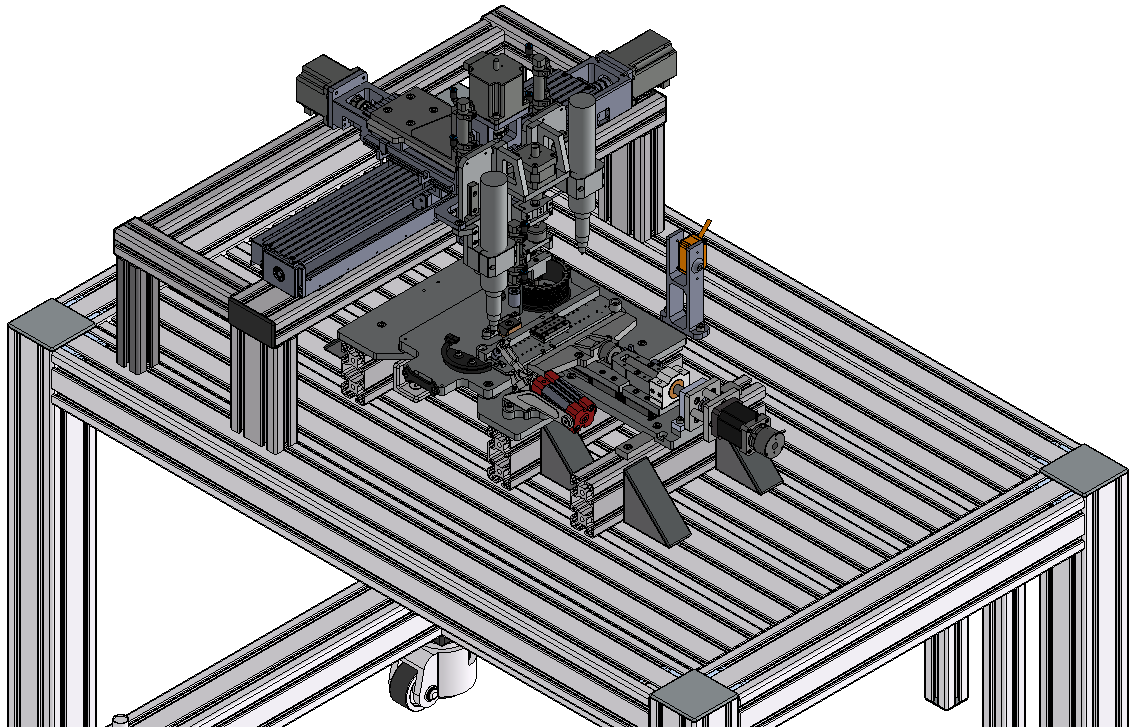
\includegraphics[width=0.95\linewidth]{Bilder/05_Konzeptumsetzung/Gesamtaufbau_CAD.png}
    \caption{Gesamtaufbau}
    \label{fig:gesamtaufbau_cad}
\end{figure}

\subsubsection{Modularer Aufbau der Teilsysteme}
Der mechanische Aufbau der Station ist modular gestaltet. Die einzelnen Funktionsbereiche sind in klar voneinander getrennte Teilsysteme untergliedert, bestehend aus der Werkstückaufnahme, der Vorspannstation, dem End-Effektor sowie dem Schraubmodul.

Diese Struktur zeichnet sich durch einen hohen Grad an Flexibilität aus. Einzelne Teilsysteme können bei Bedarf angepasst, ausgetauscht oder erweitert werden, ohne dass grundlegende Änderungen am Gesamtaufbau erforderlich sind. Zudem vereinfacht die modulare Auslegung sowohl den Aufbau der Station als auch deren spätere Wartung und Weiterentwicklung.

\subsubsection{Werkstückschnittstelle und Aufnahme}
Die Werkstückschnittstelle stellt die mechanische Verbindung zwischen dem Montagesystem und dem bestückten Werkstückträger (WST) dar. Sie ist als eigenständige Baugruppe ausgeführt und bildet die Grundlage für eine reproduzierbare Positionierung des Werkstücks während des gesamten Montageprozesses. Der Aufbau der Werkstückaufnahme erfolgt auf einer Basisplatte, die auf dem ITEM-Arbeitstisch montiert ist.

Zur Verbesserung der Zugänglichkeit wurde die Werkstückaufnahme um 80 mm gegenüber der Tischoberfläche erhöht. Diese Höhenanpassung ermöglicht eine erleichterte manuelle Platzierung und Entnahme des Werkstückträgers und verbessert die Greifbarkeit des WST im Produktionsbetrieb. Die Erhöhung wird durch den Einsatz von ITEM-Profilen realisiert, die als Distanzstruktur zwischen Arbeitstisch und Basisplatte dienen.

Die Positionierung des Werkstückträgers auf der Basisplatte erfolgt über zwei eingepresste Aufnahmebolzen. Dabei wird ein Rundbolzen sowie ein abgeflachter Bolzen verwendet. Diese Kombination gewährleistet eine eindeutige und wiederholgenaue Positionierung des WST in der Ebene, ohne eine Überbestimmung der Lagerung zu erzeugen. Durch die formschlüssige Führung über die Aufnahmebolzen ist sichergestellt, dass der Werkstückträger bei jedem Einlegen in derselben Lage und Orientierung positioniert wird.

Zur Fixierung des Werkstückträgers in vertikaler Richtung kommen zwei Spannvorrichtungen zum Einsatz, die den WST von oben gegen die Basisplatte pressen. Die Spannvorrichtungen sind so angeordnet, dass eine gleichmäßige Haltekraft auf den Werkstückträger wirkt und dieser während der nachfolgenden Prozessschritte sicher fixiert ist. Die Betätigung der Spannvorrichtungen erfolgt pneumatisch über ein Magnetventil, wodurch ein schnelles und zuverlässiges Spannen und Lösen des Werkstückträgers ermöglicht wird.

Der Bestückungsprozess beginnt mit dem manuellen Auflegen des bestückten Werkstückträgers auf die Basisplatte. Nach dem Aufsetzen auf die beiden Aufnahmebolzen wird der WST automatisch durch die Spannvorrichtungen fixiert. In diesem Zustand ist der Werkstückträger eindeutig positioniert und mechanisch gesichert, sodass die nachfolgenden Schritte des Vorspann- und Schraubprozesses unter reproduzierbaren geometrischen Bedingungen durchgeführt werden können.

Die Entnahme des Werkstückträgers erfolgt in umgekehrter Reihenfolge. Zunächst werden die Spannvorrichtungen gelöst, wodurch die Fixierung in vertikaler Richtung aufgehoben wird. Anschließend kann der Werkstückträger manuell von der Basisplatte abgehoben und aus der Station entnommen werden.

Der Gesamtaufbau der Werkstückaufnahme und die Basisplatte der Werkstückaufnahme mit den Positionier- und Spannelementen sind in Abbildung~\ref{fig:slc_vorspannen} dargestellt. Die detaillierte konstruktive Ausführung der Werkstückaufnahme ist in einer 2D-Zusammenbauzeichnung einschließlich der zugehörigen Stückliste im Anhang~\ref{anhang:Werkst.} dokumentiert.

\begin{figure}[htbp]
    \centering
    \begin{subfigure}[t]{0.48\linewidth}
        \centering
        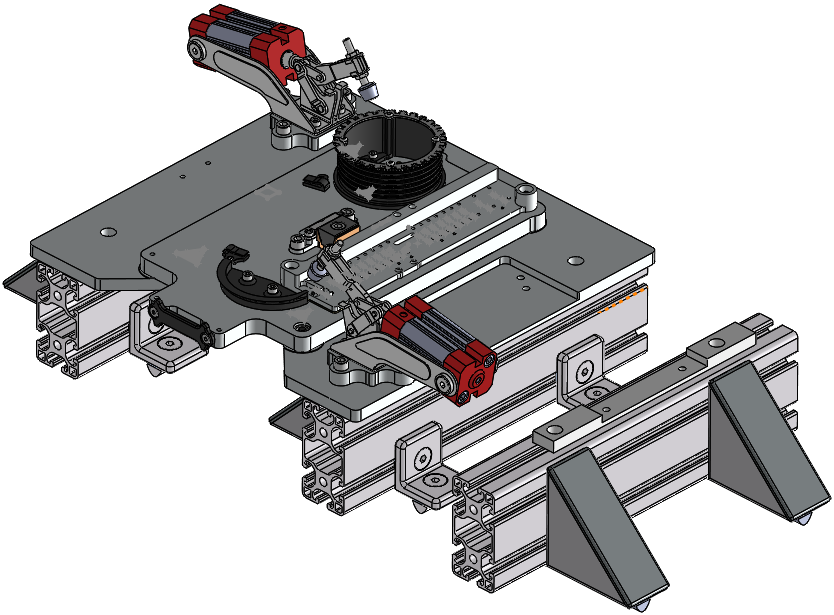
\includegraphics[width=\linewidth]{Bilder/05_Konzeptumsetzung/Werkstückaufnahme_gesamtbild.png}
        \caption{Werkstückaufnahme Gesamtbau}
        \label{fig:Werkstückaufnahme_gesamtbild_cad}
    \end{subfigure}
    \hfill
    \begin{subfigure}[t]{0.48\linewidth}
        \centering
        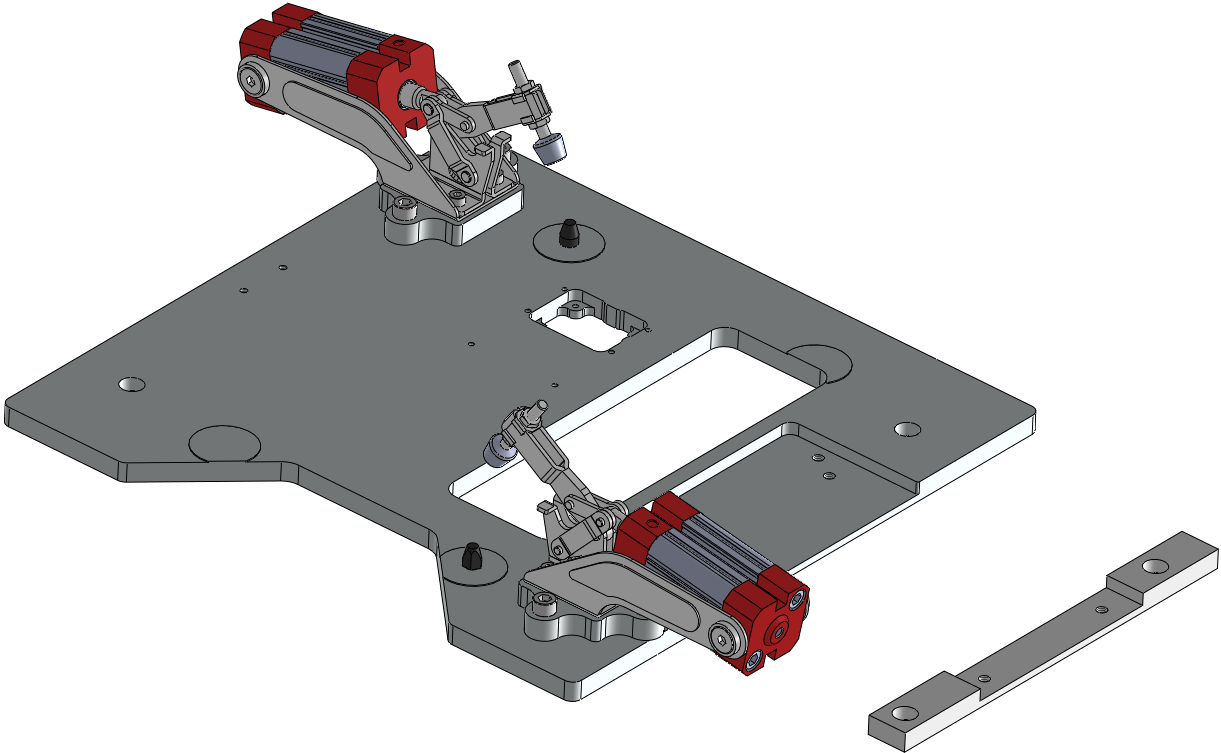
\includegraphics[width=\linewidth]{Bilder/05_Konzeptumsetzung/Werkstückaufnahme_bolzen.png}
        \caption{Basisplatte mit Positionier- und Spannelemente}
        \label{fig:Basisplatte mit Positionier- und Spannelemente}
    \end{subfigure}
    \caption{Darstellung der Werkstückaufnahme}
    \label{fig:slc_vorspannen}
\end{figure}

\subsubsection{End-Effektor (Werkzeugträger)}
Der End-Effektor bildet die zentrale mechanische Baugruppe zur Durchführung der Montageoperationen. Er ist als Werkzeugträger ausgeführt und vereint mehrere für den Aufbau der Linearführung erforderliche Funktionen innerhalb einer gemeinsamen, steifen Struktur. In den End-Effektor sind neben den beiden Schraubereinheiten sowohl das Keileinpresssystem als auch der Schlitten-Schieber integriert.

Die mechanische Grundstruktur des End-Effektors besteht aus einer tragenden Grundplatte, an der sämtliche Werkzeuge definiert positioniert und befestigt sind. Der End-Effektor ist mechanisch mit der Z-Achse der Station gekoppelt, sodass alle integrierten Werkzeuge gemeinsam verfahren werden. Dadurch bleibt die relative Lage der einzelnen Werkzeuge zueinander konstant.

Die beiden Schraubereinheiten sind symmetrisch angeordnet und ermöglichen das kontrollierte Verschrauben der Linearführung. Zur Vermeidung von Kollisionen während der Verfahrbewegungen der Gesamtstation sind beide Schrauber jeweils über pneumatische Kolbenstangenzylinder angebunden. Dadurch können die Schraubereinheiten bei Bedarf gezielt aus dem Arbeitsbereich zurückgezogen werden, bevor übergeordnete Achsbewegungen ausgeführt werden. Diese konstruktive Maßnahme erhöht die Betriebssicherheit und verhindert mechanische Kollisionen zwischen Werkzeug, Werkstück und End-Effektor.

Zentral im End-Effektor ist das Keileinpresssystem angeordnet, das mechanisch in die Grundstruktur eingebunden ist. Die zentrale Anordnung ermöglicht einen symmetrischen Kraftfluss während des Einpressvorgangs und reduziert unerwünschte Kippmomente. Das Keileinpresssystem ist zusätzlich mit zwei Gabellichtschranken ausgestattet, die als Endlagensensoren dienen und die Endpositionen des Einpressvorgangs überwachen.

Zusätzlich ist ein Schlitten-Schieber in den End-Effektor integriert, der zur definierten Positionierung einzelner Bauteile während des Montageablaufs dient. Auch dieser Schieber wird pneumatisch betätigt und ist mechanisch geführt, sodass der entsprechende Arbeitsschritt innerhalb desselben Koordinatensystems wie die übrigen Montageoperationen ausgeführt wird.

Alle drei im End-Effektor eingesetzten Rundzylinder – die beiden Zylinder für die Schraubereinheiten sowie der Zylinder für den Schlitten-Schieber – sind mit Endlagensensoren in Form von Näherungssensoren ausgestattet. Diese dienen der Überwachung der jeweiligen Endpositionen und können sicher stellen, dass übergeordnete Bewegungen der Station nur dann freigegeben werden, wenn sich alle Werkzeuge in einer kollisionsfreien Position befinden.

Bei der Auslegung des End-Effektors wurde besonderer Wert auf eine hohe Steifigkeit gelegt. Während des Schraub- und Einpressvorgangs wirken sowohl axiale als auch laterale Kräfte auf die Struktur. Relativbewegungen zwischen End-Effektor, Werkzeugen und Werkstück müssen daher möglichst gering gehalten werden, da sie sich unmittelbar auf die Montagequalität auswirken können. Die kompakte Bauweise sowie kurze Kraftflussketten tragen dazu bei, Verformungen zu minimieren und eine hohe Wiederholgenauigkeit zu gewährleisten.

Abbildung~\ref{fig:EE_iso} zeigt den End-Effektor in isometrischer Darstellung mit integrierten Schraubereinheiten, Keileinpresssystem und Schlitten-Schieber. In dieser Ansicht ist insbesondere die Anbindung der Schraubereinheiten an die pneumatischen Rundzylinder erkennbar.

Die detaillierte konstruktive Ausführung des End-Effektors ist in einer 2D-Zusammenbau\-zeichnung einschließlich der zugehörigen Teil-Stückliste im Anhang~\ref{anhang:ee_2d} dokumentiert. Die Ansteuerung der pneumatischen Zylinder sowie die Auswertung der Endlagensensoren werden in den Abschnitten zur \enquote{Aktorik und Antriebstechnik} (vgl. Abschnitt~\ref{sec:aktorik_antrieb}) sowie zur \enquote{Sensorik und Messtechnik} (vgl. Abschnitt~\ref{sec:sensorik_messtechnik}) behandelt.

\begin{figure}[H]
    \centering
    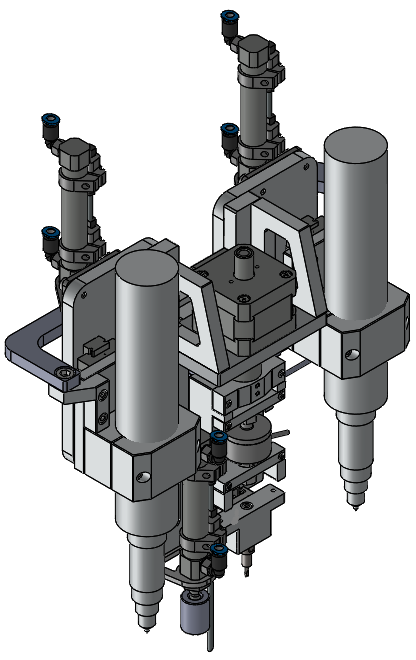
\includegraphics[width=0.40\linewidth]{Bilder/05_Konzeptumsetzung/End effektor iso anschicht.png}
    \caption{Isometrische Ansicht des End Effektors}
    \label{fig:EE_iso}
\end{figure}

\subsubsection{Achssystem}
Das Achssystem übernimmt die Positionierung des End-Effektors relativ zur Werkstückaufnahme und bildet die Grundlage für alle translatorischen Bewegungen innerhalb des Montagesystems. Es ist als kartesisches System ausgeführt und auf einem ITEM-Gestell montiert, das die notwendige Steifigkeit und Zugänglichkeit für den Montageprozess bereitstellt.

Als Linearachsen kommen GKS-Achsen der Firma GMT Europe zum Einsatz. Die Achsen sind modular aufgebaut und über Adapterplatten miteinander verbunden. Diese Adapterplatten dienen als definierte mechanische Schnittstellen zwischen den einzelnen Achsen sowie zwischen Achssystem und End-Effektor. Durch die Verwendung von Adapterplatten wird eine präzise Ausrichtung der Achsen zueinander gewährleistet und der mechanische Integrationsaufwand reduziert.

Das Achssystem ist vollständig auf dem ITEM-Gestell aufgebaut, wie in Abbildung~\ref{fig:roboter} dargestellt. Das Gestell übernimmt dabei sowohl die Funktion der tragenden Struktur als auch die Einbindung des Achssystems in den Gesamtaufbau der Station. Die offene Bauweise des ITEM-Gestells erleichtert zudem den Zugang für Montage-, Wartungs- und Servicearbeiten.

Alle eingesetzten Achsen sind mit Endlagensensoren ausgestattet. Pro Achse kommen jeweils zwei Gabellichtschranken zum Einsatz, die die Endpositionen der Verfahrbewegung absichern. Dadurch wird sichergestellt, dass die Bewegungen der Achsen ausschließlich innerhalb definierter mechanischer Grenzen erfolgen. Die Endlagensensoren dienen sowohl der Referenzierung als auch zum Schützen des Achssystems.

Die mechanische Auslegung des Achssystems ist auf eine hohe Wiederholgenauigkeit ausgelegt. Die Führung der Achsen sowie deren Anbindung über Adapterplatten sorgen für eine stabile Kraftübertragung und minimieren Relativbewegungen zwischen den einzelnen Baugruppen. Damit bildet das Achssystem die Grundlage für die präzise Positionierung des End-Effektors während des Vorspann-, Einpress- und Schraubprozesses.

Die detaillierte konstruktive Ausführung des Achssystems ist in einer 2D-Zusammenbau\-zeichnung einschließlich der zugehörigen Teil-Stückliste im Anhang~\ref{anhang:achssystem} dokumentiert.

Die Ansteuerung der Achsen sowie die Auswertung der Endlagensensoren werden in den Abschnitten zur \enquote{Aktorik und Antriebstechnik} (vgl. Abschnitt~\ref{sec:aktorik_antrieb}) sowie zur \enquote{Sensorik und Messtechnik} (vgl. Abschnitt~\ref{sec:sensorik_messtechnik}) behandelt.

\begin{figure}[H]
    \centering
    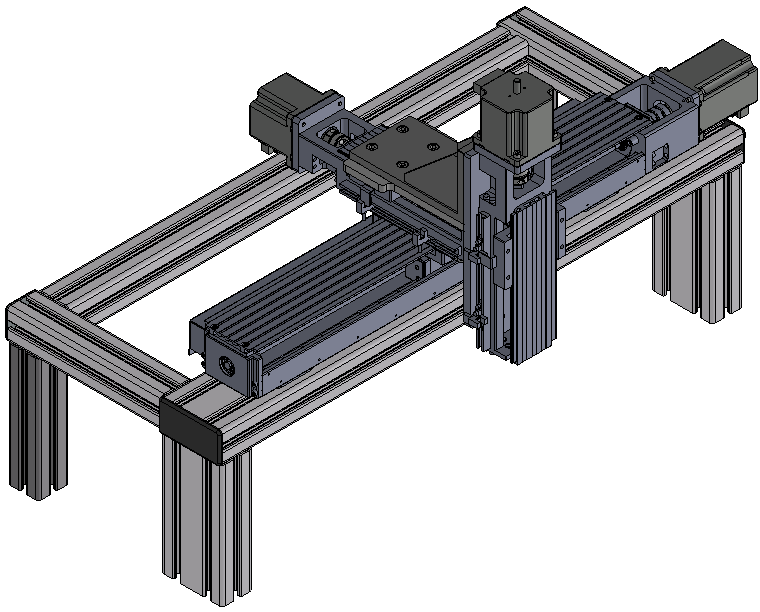
\includegraphics[width=0.45\linewidth]{Bilder/05_Konzeptumsetzung/Achssystem.png}
    \caption{Achssystem}
    \label{fig:roboter}
\end{figure}

\subsection{Aktorik und Antriebstechnik}
\label{sec:aktorik_antrieb}
\subsubsection{Eingesetzte Aktoren}
In diesem Abschnitt werden die im Montagesystem eingesetzten Aktoren beschrieben, deren Auswahl und Integration Bestandteil dieser Arbeit sind. Der Fokus liegt dabei auf den Linearachsen mit zugehörigen Motoren, den Schraubereinheiten sowie den pneumatischen Aktoren für Bewegungs- und Spannfunktionen.

Die Antriebe des Vorspannsystems sowie des Keileinpresssystems wurden nicht neu ausgelegt. Diese Systeme waren bereits als funktionsfähige und erprobte Lösungen vorhanden und wurden als Stand der Technik übernommen. Sie werden daher in diesem Kapitel nicht ausgelegt.

Für die Positionieraufgaben im System werden drei Linearachsen eingesetzt. Die Auswahl der Achsen sowie der zugehörigen Schrittmotoren erfolgte im Rahmen dieser Arbeit auf Basis der geforderten Verfahrwege, der zu bewegenden Massen sowie der erforderlichen Positioniergenauigkeit.

Als Schraubwerkzeuge kommen elektrische Schrauber des Herstellers Kolver zum Einsatz, die bereits im Unternehmen verfügbar sind. Diese wurden gezielt in das Montagekonzept integriert. Ergänzend dazu werden pneumatische Rundzylinder für einfache lineare Bewegungen sowie eine vorhandene Spannvorrichtung zur Fixierung der Bauteile eingesetzt.

Tabelle~\ref{tab:aktoren_uebersicht} fasst die Aktoren hinsichtlich Typ, Funktion und Einsatzbereich zusammen.\cite{ds_gmt_gka_gks,ds_nanotec_sca5618,ds_nanotec_scb6018,ds_kolver_mito15ca,ds_kolver_nato50ca,ds_kolver_edu2ae,ds_festo_dsnu,ds_gn860}

\begin{table}[H]
\centering
\small
\setlength{\tabcolsep}{4pt}
\renewcommand{\arraystretch}{1.2}
\begin{tabular}{|p{3.0cm}|p{4.8cm}|p{4.0cm}|p{2.8cm}|}
\hline
\textbf{Aktor} & \textbf{Typ / Bezeichnung} & \textbf{Funktion im System} & \textbf{Zuordnung} \\
\hline
Linearachse X & GKA4270-500-12N-P10 & Positionierung in X-Richtung & Positionierachse \\
\hline
Linearachse Y & GKS3060-50-12N-P5 & Positionierung in Y-Richtung & Positionierachse \\
\hline
Linearachse Z & GKS3060-50-12N-P5 & Positionierung in Z-Richtung & Positionierachse \\
\hline
Schrittmotor X & Nanotec SCA5618L4204-B2 & Antrieb der X-Achse & Elektrischer Antrieb \\
\hline
Schrittmotor Y/Z & Nanotec SCB6018M4204-B & Antrieb der Y- und Z-Achse & Elektrischer Antrieb \\
\hline
Schrauber SLC-24 & MITO15CA & Verschrauben von M2-Schrauben & Prozessaktor \\
\hline
Schrauber SLC-17 & NATO50CA/TA & Verschrauben von M1{,}4-Schrauben & Prozessaktor \\
\hline
Pneumatikzylinder & DSNU-S-12-40-P-MQ & Bewegung der Schraubereinheiten und des Schlitten-Schiebers & Hilfsaktor \\
\hline
Spannvorrichtung & GN 860-75-CP-M & Fixierung des Werkstückträgers während der Montage & Spanntechnik \\
\hline
\end{tabular}
\caption{Übersicht der eingesetzten Aktoren und deren funktionale Zuordnung}
\label{tab:aktoren_uebersicht}
\end{table}

\subsubsection{Achssysteme}
Die Achssysteme übernehmen im Montagesystem ausschließlich Positionieraufgaben. Für diesen Zweck wurden vorkonfigurierte Linearachsen ausgewählt, die von GMT Europe bezogen wurden. Alle Achsen arbeiten mit Kugelgewindetrieben und sind jeweils einem eigenen Schrittmotor zugeordnet.

Die X-Achse wird durch eine Linearachse des Typs GKA4270-500-12N-P10 realisiert. Sie besitzt einen effektiven Verfahrweg von 413\,mm und dient der horizontalen Positionierung der Funktionseinheiten. Aufgrund der vergleichsweise großen Verfahrstrecke wurde diese Achse mit einer Spindelsteigung von 10\,mm ausgeführt, um eine ausreichende Verfahrgeschwindigkeit bei gleichzeitig robuster Kraftübertragung zu gewährleisten. Die hohe dynamische und statische Tragfähigkeit der Achse stellt sicher, dass die im Betrieb auftretenden Lasten mit ausreichender Sicherheitsreserve innerhalb der zulässigen Grenzwerte liegen \cite{ds_gmt_gka_gks}.

Für die Y- und Z-Achse werden Linearachsen des Typs GKS3060-50-12N-P5 eingesetzt. Diese Achsen besitzen einen Verfahrweg von jeweils 50\,mm und sind für kurze, präzise Zustellbewegungen ausgelegt. Die geringere Spindelsteigung von 5\,mm ermöglicht eine höhere Auflösung und eine feinere Positionierung, was insbesondere für die Zustellbewegung der Schraubereinheiten relevant ist. Auch hier liegen die zulässigen Lasten der Achsen deutlich über den im Prozess auftretenden Belastungen \cite{ds_gmt_gka_gks}.

Als Antriebe kommen Schrittmotoren des Herstellers Nanotec zum Einsatz. Die X-Achse wird von einem Motor des Typs SCA5618L4204-B2 mit einem Haltemoment von 230\,Ncm angetrieben. Für die Y- und Z-Achse werden Motoren des Typs SCB6018M4204-B mit einem Haltemoment von 200\,Ncm verwendet. Alle Motoren besitzen einen Schrittwinkel von 1{,}8° und damit 200 Vollschritte pro Umdrehung \cite{ds_nanotec_sca5618,ds_nanotec_scb6018}.

Aus der Kombination von Schrittwinkel, eingestellter Microstepping-Auflösung und Spindelsteigung ergibt sich für alle drei Achsen eine theoretische lineare Auflösung von \qty{1,56}{\micro\meter} pro Microstep. Die eingesetzte Trinamic-Motorsteuerung unterstützt diese Microstepping-Betriebsart hardwareseitig. Ein Mikroschritt stellt dabei eine elektronisch geregelte Unterteilung eines Vollschrittes dar, wodurch eine feinere Positionsauflösung sowie ein ruhigerer Motorlauf erreicht werden. Dieser Wert liegt deutlich unterhalb der in der Anforderungsliste definierten Toleranz von \qty{15}{\micro\metre} und erfüllt damit die Anforderungen an die Positionierauflösung der Achssysteme. Rechnerisch wären hierfür bereits 4 Microsteps pro Vollschritt für die X-Achse sowie 2 Microsteps pro Vollschritt für die Y- und Z-Achse ausreichend. Die tatsächlich gewählten Einstellungen von 32 Microsteps für die X-Achse sowie 16 Microsteps für die Y- und Z-Achse stellen somit eine zusätzliche Reserve hinsichtlich Auflösung und Laufruhe dar. Die zugehörigen Berechnungen zur Schrittauflösung sind in Anhang~\ref{anhang:berechnungen} dargestellt.

Auf der Grundlage der durchgeführten Auslegungs- und Plausibilitätsberechnungen wurden für die Achsen maximale lineare Geschwindigkeiten von etwa \qty{23,8}{\mm\per\s} sowie maximale Beschleunigungen von rund \qty{182}{\mm\per\s\tothe{2}} festgelegt. Diese berechneten Sollwerte wurden anschließend durch eine geeignete Wahl der Steuerungsparameter umgesetzt. Daraus resultieren bei idealisierter Betrachtung reine Fahrzeiten von etwa \qty{17}{\second} für den vollen X-Verfahrweg sowie rund \qty{2}{\second} für einen 50-mm-Hub auf der Y- und Z-Achse. Die detaillierten Berechnungen zu Geschwindigkeit, Beschleunigung und Fahrzeit sind im Anhang~\ref{anhang:berechnungen} aufgeführt.

Zur Vermeidung von Schrittverlusten wurde die Motorauswahl zusätzlich über den erforderlichen Drehmomentbedarf überprüft. Aus den maximalen Achsgeschwindigkeiten ergeben sich Motordrehzahlen von etwa \qty{143}{\per\minute} für die X-Achse sowie \qty{286}{\per\minute} für die Y- und Z-Achse. Die Berechnung der notwendigen Antriebsmomente zeigt, dass diese deutlich unterhalb der bei diesen Drehzahlen verfügbaren Pull-out-Momente der eingesetzten Motoren liegen. Das Pull-out-Moment beschreibt dabei das maximal verfügbare Drehmoment eines Schrittmotors bei einer gegebenen Drehzahl, bei dem der Motor dem vorgegebenen Schrittsignal noch synchron folgen kann, ohne Schritte zu verlieren. Dabei wurde neben dem Haltemoment auch der Drehzahlbereich berücksichtigt, in dem die Achsen im Betrieb bewegt werden. Somit ist sichergestellt, dass die Motoren auch unter Last zuverlässig arbeiten und es nicht zu Schrittverlusten kommt. Der vollständige Drehmomentnachweis ist in Anhang~\ref{anhang:berechnungen} dokumentiert.

Die vollständigen Berechnungen zur Auflösung, Geschwindigkeit, Beschleunigung sowie zum Drehmomentnachweis sind zusammenfassend im Anhang~\ref{anhang:berechnungen} detailliert dokumentiert.


\subsubsection{Pneumatische Aktoren}
Pneumatische Aktoren werden im Montagesystem gezielt für unterstützende Bewegungen eingesetzt, bei denen keine hochgenaue Positionierung erforderlich ist. Ihr Einsatz dient insbesondere der Prozessentkopplung und der Reduktion zusätzlicher Bewegungen der elektrischen Achssysteme.

Für diese Aufgaben werden drei pneumatische Rundzylinder des Typs DSNU-S-12-40-P-MQ von Festo eingesetzt. Zwei dieser Zylinder sind den Schraubereinheiten zugeordnet. Sie sorgen dafür, dass die Schrauber beim Ansetzen der Schrauben definiert und mit ausreichender Kraft in Richtung des Schraubenkopfes zugestellt werden. Dadurch wird sichergestellt, dass der Schrauber korrekt im Schraubenkopf sitzt und ein unerwünschtes \enquote{Freidrehen} des Werkzeugs vermieden wird. Diese pneumatische Zustellbewegung unterstützt somit direkt die Prozesssicherheit des Schraubvorgangs.\cite{ds_festo_dsnu}

Der dritte pneumatische Zylinder wird für die Bewegung des Schlitten-Schiebers verwendet. Auf eine zusätzliche Bewegung des gesamten Endeffektors in Z-Richtung kann dadurch verzichtet werden, was den Bewegungsablauf vereinfacht und die mechanische Belastung der Achssysteme reduziert.

Die eingesetzten Rundzylinder besitzen einen Kolbendurchmesser von 12 mm und einen Hub von 40 mm. Bei einem Betriebsdruck von \qty{0,6}{\mega\pascal} ergibt sich eine theoretische Zylinderkraft von rund \qty{68}{\newton}, die für die beschriebenen Bewegungsaufgaben ausreichend ist.\cite{ds_festo_dsnu}

Zusätzlich wird eine vorhandene Spannvorrichtung des Typs GN 860-75-CP-M eingesetzt. Diese dient der Fixierung des Werkstückträgers während des Schraubprozesses und stellt sicher, dass die Bauteile während der Montage lagegenau gehalten werden. Die Spannvorrichtung wurde ohne konstruktive Änderungen in das System integriert.\cite{ds_gn860}

Durch den gezielten Einsatz pneumatischer Aktoren für diese unterstützenden Funktionen kann sich die elektrische Antriebstechnik auf präzise Positionieraufgaben konzentrieren. Dies trägt zu einem übersichtlichen Systemaufbau sowie zu einer robusten und prozesssicheren Umsetzung der Montageabläufe bei.

\subsubsection{Schraubeinheiten}
Die Schraubereinheiten stellen zentrale Prozessaktoren des Montagesystems dar und sind maßgeblich für die Montagequalität verantwortlich. Abhängig von der Baugröße des Positionierers kommen unterschiedliche Schraubermodelle zum Einsatz.

Für Positionierer der Baugröße SLC-24 mit M2-Schrauben wird ein Schrauber des Typs MITO15CA verwendet. Dieser deckt einen Drehmomentbereich von 0,35 Nm bis 1,5 Nm ab und arbeitet mit Drehzahlen zwischen 450 und 850 $\min^{-1}$. Für Positionierer der Baugröße SLC-17 mit M1,4-Schrauben kommt ein Schrauber des Typs NATO50CA/TA zum Einsatz, dessen Drehmomentbereich zwischen 0,05 Nm und 0,7 Nm liegt.\cite{ds_kolver_nato50ca, ds_kolver_mito15ca}

Die Schrauber werden über externe Controller der EDU2AE-Serie betrieben und über digitale Ein- und Ausgänge in die Anlagensteuerung eingebunden. Die Anzahl der Schrauben pro Montage variiert in Abhängigkeit von der Länge und Breite des jeweiligen Positionierers, was durch die flexible Prozessführung berücksichtigt wird.\cite{ds_kolver_edu2ae}

Die Schrauber sind mechanisch an die jeweiligen Z-Achsen angebunden. Die Zustellbewegung erfolgt ausschließlich entlang der Z-Achse.

\subsubsection{Zusammenfassung der Antriebsauslegung}
Die im Rahmen dieser Arbeit ausgewählte Aktorik deckt alle erforderlichen Bewegungs- und Montagefunktionen des Systems zuverlässig ab. Die Kombination aus elektrisch angetriebenen Linearachsen für präzise Positionieraufgaben und pneumatischen Aktoren für Hilfs- und Spannfunktionen hat sich als zweckmäßig und übersichtlich erwiesen.

Die Achssysteme und Motoren verfügen über ausreichende Leistungsreserven, sodass ein stabiler Betrieb auch bei variierenden Prozessbedingungen gewährleistet ist. Bestehende Antriebslösungen für das Vorspannsystem und das Keileinpresssystem wurden bewusst übernommen, um auf erprobte Konzepte zurückzugreifen und den Fokus der Arbeit auf die Auslegung der Positionier- und Schraubprozesse zu legen.

\subsection{Sensorik und Messtechnik}
\label{sec:sensorik_messtechnik}

\subsubsection{Ziel der Sensorik}
Die Sensorik dient der Überwachung von Positionen, Kräften und Zuständen innerhalb des Montageprozesses. Ziel ist es, eine sichere und reproduzierbare Durchführung der einzelnen Prozessschritte zu gewährleisten sowie fehlerhafte Zustände frühzeitig zu erkennen. Die Sensoren werden dabei primär zur Referenzierung, Prozessfreigabe und Plausibilitätsprüfung eingesetzt und tragen wesentlich zur Erhöhung der Prozesssicherheit bei.

\subsubsection{Positions- und Referenzsensoren}
Zur Referenzierung und Endlagenüberwachung der motorisierten Achsen sind an allen Linearachsen jeweils zwei Gabellichtschranken des Typs Panasonic PM-F25 eingesetzt. Der in Motornähe montierte Sensor dient zur Referenzfahrt und definiert den Nullpunkt der jeweiligen Achse. Der zweite Sensor übernimmt die Funktion der Endlagenüberwachung und verhindert unzulässige Verfahrbewegungen.\cite{ds_panasonic_pmf25}

Die Sensoren sind direkt an den Linearachsen montiert. Im Vorspannsystem waren ursprünglich keine Endlagensensoren vorgesehen; diese wurden im Rahmen dieser Arbeit ergänzend an der Adapterplatte nachgerüstet. Auch im Keileinpresssystem sind Endlagensensoren an der Adapterplatte angebracht, deren mechanische Integration bereits im Vorfeld erfolgte. Die Endlagensensoren sind als digitale Schaltsensoren ausgeführt und elektrisch angebunden.

An den eingesetzten Rundzylindern werden jeweils zwei Näherungssensoren zur Erfassung der Kolbenendlagen verwendet. Hier kommen Sensoren des Typs Festo SMT-8M-A-PS-24V-E-0,3-M8D zum Einsatz, die mithilfe von Festo SMBR 8-12 Haltern direkt am Zylinder montiert sind. Diese Sensoren ermöglichen eine zuverlässige Zustandsüberwachung der pneumatischen Bewegungen und dienen ebenfalls der Prozessfreigabe.\cite{ds_festo_smt8m, ds_festo_smbr}

\subsubsection{Kraftmesstechnik}
Zur Überwachung der aufgebrachten Kräfte sind in der Vorspannmechanik sowie im Keileinpresssystem Kraftmessdosen integriert. Die verwendeten Sensoren waren Bestandteil eines bestehenden Systems und wurden im Rahmen dieser Arbeit übernommen. Im Keileinpresssystem wird eine Kraftmessdose des Typs KM26z-50N eingesetzt, während in der Vorspannmechanik eine Kraftmessdose des Typs KM26z-500N verwendet wird.\cite{ds_km26z_50n, ds_km26z_500n}

Die Kraftmessdosen sind jeweils zwischen Aktor und mechanischer Struktur angeordnet, sodass die tatsächlich eingeleitete Kraft direkt erfasst werden kann. Die Sensorsignale werden analog ausgegeben und über externe Messverstärker des Typs ME-Meßsysteme GSV-1H 010/250/2 aufbereitet. Diese Verstärker wurden im Zuge dieser Arbeit ergänzt, da sie im ursprünglichen System nicht vorhanden waren. Die erfassten Kraftwerte dienen dem Vergleich von Soll- und Ist-Kraft und ermöglichen eine Überwachung der eingestellten Vorspannung während des Montageprozesses.\cite{ds_me_gsv1h}

\subsubsection{Optische Messtechnik}
Zur berührungslosen Erfassung der Schlittenposition wird ein Laser-Triangulationssensor des Typs Micro-Epsilon optoNCDT 1220 mit einem Messbereich von 500 mm eingesetzt. Der Sensor misst die Schlittenposition in X-Richtung und ermöglicht eine präzise Bestimmung der Lage während des Montageablaufs. Die Wiederholgenauigkeit beträgt \qty{50}{\micro\metre}. Die Linearitätsabweichung des Laser-Triangulationssensors liegt im zentralen Messbereich ($< \qty{750}{\micro\metre}$) unter \num{0,15}\,\% des Full-Scale-Outputs (FSO) und beträgt über den gesamten Messbereich bis \qty{1500}{\micro\metre} maximal \num{0,30}\,\% FSO.

Der Einsatz eines Laser-Triangulationssensors ist insbesondere aufgrund der sehr kleinen verfügbaren Messoberfläche erforderlich. Als Messziel dient der Schraubenkopf des Schlittens mit einem Durchmesser von etwa 4 mm, wodurch taktile Messverfahren nur eingeschränkt geeignet wären. Die Signalausgabe erfolgt analog über eine $4\text{--}20\text{ mA}$-Schnittstelle und wird von der Steuerung zur Positionsüberwachung und Plausibilitätsprüfung genutzt.\cite{ds_microepsilon_optoncdt1220}

\subsection{Steuerungskonzept}
\subsubsection{Grundidee der Steuerungsarchitektur}
Die Steuerungsarchitektur basiert auf einer funktionalen Trennung zwischen Bewegungssteuerung und übergeordneter Prozess- und Ablaufsteuerung. Die Ansteuerung der motorisierten Achsen erfolgt über einen Trinamic TMCM-6110 Motorkontroller, während die Einbindung der Peripherie sowie die Prozesslogik über ein modulares WAGO-I/O-System realisiert wird. Diese Aufteilung ermöglicht eine übersichtliche Struktur, reduziert die Komplexität der Einzelkomponenten und erleichtert eine spätere Erweiterung des Systems.

Der Einsatz des WAGO-Systems wurde erforderlich, da die am TMCM-6110 verfügbaren Ein- und Ausgänge für die vollständige Anbindung aller Aktoren und Sensoren nicht ausreichten. Durch die Kombination beider Systeme konnte eine klare Trennung zwischen Bewegungsfunktionen und prozessrelevanten Ein- und Ausgängen umgesetzt werden.

Zur übersichtlichen Darstellung der Ein- und Ausgänge sowie der angebundenen Aktoren und Sensoren ist in Abbildung~\ref{fig:sys_archi} ein Blockdiagramm dargestellt. Es zeigt die Zuordnung der Peripheriekomponenten zum TMCM-6110 sowie die Anbindung des Rechners und des WAGO-I/O-Systems. Die vollständigen elektrischen Schaltpläne sind im Anhang~\ref{anhang:schaltplan} abgelegt und dienen dort der detaillierten Nachvollziehbarkeit und Referenz.

\begin{figure}[H]
    \centering
    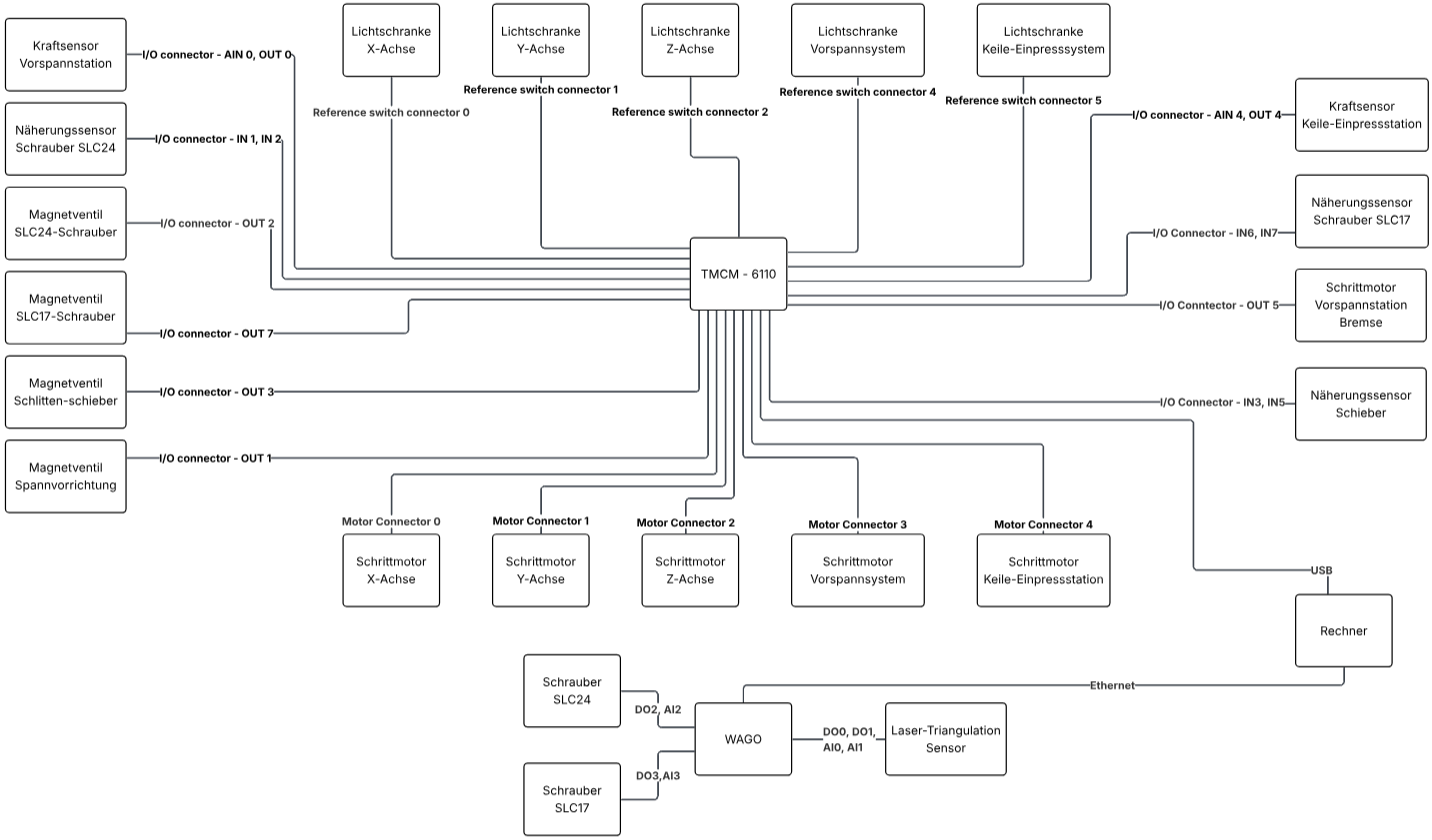
\includegraphics[width=1\linewidth]{Bilder/05_Konzeptumsetzung/Systemarchi.png}
    \caption{I/O-Belegung und Systemübersicht}
    \label{fig:sys_archi}
\end{figure}

\subsubsection{Einbindung der Aktoren}
Alle fünf eingesetzten Motoren sind direkt an die Motorkontroller-Ausgänge des TMCM-6110 angebunden. Die zugehörigen Endlagensensoren sind an den dafür vorgesehenen Referenz- und Endschalter-Eingängen des Motorkontrollers angeschlossen und dienen der Referenzfahrt sowie der Endlagenüberwachung.

Die Ansteuerung der pneumatischen und elektrischen Aktoren erfolgt über digitale Ausgänge. Dazu zählen eine Bremse für den Motor des Vorspannsystems, vier Magnetventile für die beiden Schraubereinheiten, den Schlittenschieber sowie die Spannvorrichtung. Zusätzlich sind zwei digitale Ausgänge zur Tara-Funktion der Kraftmessverstärker vorgesehen. Diese Ausgänge ermöglichen das gezielte Zurücksetzen der Kraftmesssignale vor Beginn eines Messvorgangs. Die Tara-Funktionen der Kraftmessverstärker sind ebenfalls über Relais angebunden. Hintergrund ist, dass die digitalen Ausgänge des TMCM-6110 als Open-Drain-Ausgänge ausgeführt sind, während die eingesetzten Kraftmessverstärker ein +24-V-Signal zur Auslösung der Tara-Funktion benötigen. Die Relais dienen hierbei zur galvanischen Trennung sowie zur Anpassung der Signalpegel zwischen dem Motorkontroller und dem Verstärkereingang.\cite{man_trinamic_tmcm6110}

\subsubsection{Einbindung der Sensoren}
Die Näherungssensoren der Rundzylinder sind als digitale Eingänge ausgeführt. Insgesamt sind sechs digitale Eingänge belegt, wobei pro Rundzylinder jeweils zwei Sensoren zur Erfassung der Endlagen eingesetzt werden.

Die Kraftmessdosen werden über analoge Eingänge angeschlossen. Die verstärkten Kraftsignale der beiden Messstellen werden an zwei analoge Eingänge des Systems geleitet und dienen der Überwachung der aufgebrachten Kräfte im Vorspann- und Keileinpressprozess.

Der Laser-Triangulationssensor ist ebenfalls über einen analogen Eingang angebunden und liefert sein Messsignal als $4\text{--}20\text{ mA}$-Stromsignal. Zusätzlich werden Status- und Fehlerinformationen des Lasers sowie Rückmeldesignale der Schrauber als digitale Signale erfasst.

\subsubsection{WAGO-I/O-System}
Das WAGO-I/O-System ist modular aufgebaut und besteht aus einem Modbus-Koppler des Typs WAGO 750-362, einer Potentialeinspeisung WAGO 750-602 sowie mehreren Ein- und Ausgangsmodulen. Zur Ansteuerung der Aktoren wird ein digitales Ausgangsmodul WAGO 750-531 eingesetzt. Die Erfassung der analogen Sensorsignale erfolgt über zwei analoge Eingangsmodule des Typs WAGO 750-466. Den Abschluss des Systems bildet ein Endmodul WAGO 750-600.\cite{ds_wago_750362, ds_wago_750602, ds_wago_750531, ds_wago_750466, ds_wago_750600}

An die digitalen Ausgänge des WAGO-Systems sind die Ein- und Ausschaltung des Lasers sowie dessen Funktionseingang jeweils über Relais angebunden. Darüber hinaus werden die Startsignale der beiden Schrauber (MITO15CA und NATO50CA/TA) über Relais geschaltet. Während das WAGO-Ausgangsmodul beim Aktivieren eines digitalen Ausgangs ein +24-V-Signal liefert, erwarten die angeschlossenen Geräte ein Open-Drain- bzw. potenzialfreies Schaltsignal. Die Relais übernehmen in diesem Fall die notwendige Signalumsetzung und stellen eine kompatible Anbindung der Komponenten sicher. Die analogen Eingänge erfassen das Stromsignal des Lasersensors. Status- und Rückmeldesignale der Schrauber sowie das Fehlerausgangssignal des Lasers werden als digitale Signale ausgewertet.

\subsection{Ablaufverfahren und zeitliche Auslegung des Prozesses}
Im Folgenden wird der konzeptionell vorgesehene Montageablauf des Systems beschrieben. 
Zusätzlich werden für die einzelnen Prozessschritte berechnete Zeitanteile angegeben, um die zeitliche Machbarkeit des Gesamtkonzepts zu bewerten.

\begin{longtable}{|c|p{7.5cm}|c|p{3.5cm}|}
\hline
\textbf{Nr.} & \textbf{Prozessschritt} & \textbf{Zeit [s]} & \textbf{Achsen / Aktoren} \\
\hline
\endfirsthead

\hline
\endhead
\endfoot
\endlastfoot

1 &
Synchrones Verfahren aller Achsen von Referenz- in Startposition (X mittig positioniert, Y auf hintere Führung ausgerichtet) &
6.0 &
X, Y, Z (überlagert) \\
\hline

2 &
Einleiten des Vorspannvorgangs &
3.5 &
Vorspannaktor \\
\hline

3 &
Positionierung der Z-Achse zur ersten Schraubposition &
1.0 &
Z \\
\hline

4 &
Verschraubung der ersten Schraube mit automatischem Schrauber (MITO); geringfügige Korrekturbewegungen zur exakten Ausrichtung &
2.0 &
Schrauber, X/Y (fein) \\
\hline

5 &
Aktivierung des Schiebers und Verschieben des Schlittens zur Vorbereitung der nächsten Schraubposition &
2.2 &
Schieberaktor \\
\hline

6 &
Positionierung zur zweiten Schraubposition durch geringe Korrekturbewegungen &
1.0 &
X, Y \\
\hline

7 &
Verschraubung der zweiten Schraube mit automatischem Schrauber &
2.0 &
Schrauber \\
\hline

8 &
Erneutes Verschieben des Schlittens mittels Schieber zur Vorbereitung der dritten Schraubposition &
1.2 &
Schieberaktor \\
\hline

9 &
Positionierung zur dritten Schraubposition durch geringe Achskorrekturen &
2.0 &
X, Y \\
\hline

10 &
Verschraubung der dritten Schraube &
2.0 &
Schrauber \\
\hline

11 &
Synchrones Verfahren aller Achsen in Referenzposition &
6.0 &
Schrauber \\
\hline

\multicolumn{2}{|r|}{\textbf{Gesamte berechnete Prozesszeit}} &
\textbf{28.8} &
Ohne Nebenzeiten \\
\hline
\caption{Ablauf und berechnete Prozesszeiten des Montageprozesses für SLC-2445}
\label{tab:prozesszeiten_slc2445} \\
\end{longtable}


Die in Tabelle~\ref{tab:prozesszeiten_slc2445} dargestellten Zeiten basieren auf den berechneten Verfahrwegen der Achssysteme, den parametrierten Geschwindigkeiten sowie den funktional notwendigen Halte- und Prozesszeiten der einzelnen Montageoperationen. 

Die Tabelle verdeutlicht den logischen Ablauf des Montageprozesses von der Positionierung des Werkstückträgers über das Vorspannen der Linearführung bis hin zum finalen Schraubprozess. Gleichzeitig zeigt sie, dass der gesamte Aufbauprozess innerhalb einer realistischen und für eine spätere Automatisierung geeigneten Zykluszeit liegt.

\subsection{Gesamtstückliste}
Die Gesamtstückliste fasst alle wesentlichen Komponenten des entwickelten Montagesystems zusammen und dient der strukturierten Dokumentation des Systemaufbaus. Sie ermöglicht eine nachvollziehbare Zuordnung der eingesetzten Baugruppen zu den jeweiligen Teilfunktionen und bildet die Grundlage für eine spätere Erweiterung oder Reproduktion des Systems.

Im Hauptteil der Arbeit wird bewusst auf eine detaillierte Auflistung einzelner Bauteile verzichtet. Stattdessen werden ausschließlich die Hauptkomponenten berücksichtigt, die für das funktionale Verständnis des Systems relevant sind. Die vollständige und detaillierte Gesamtstückliste ist im Anhang~\ref{tab:gesamt_stueckliste} enthalten.

Die Stückliste ist in die Bereiche Mechanik, Aktorik, Sensorik sowie Steuerung und Elektrik gegliedert. Neben den mechanischen Baugruppen und Aktoren umfasst sie auch die zentralen Steuerungskomponenten, darunter den Motorkontroller, das modulare WAGO-I/O-System, Kraftmessverstärker sowie Relais zur Signalpegelanpassung zwischen unterschiedlichen Ein- und Ausgangslogiken. Ebenfalls enthalten sind die wesentlichen Sensoren zur Positions-, Kraft- und Zustandsüberwachung.